\tjformsection{一、\tjheadertext 课题背景}
%\tjformnote{根据实际情况写为毕业设计或毕业论文，下同（此项成稿删除）}

\tjformsubsection{1．课题来源及研究的目的和意义}

\textbf{课题来源：}本课题来源于指导教师课题组在视觉语言动作模型（Vision-Language-Action, VLA）实时推理方向的研究工作。该课题基于预训练VLA模型（如\(\pi_{0.5}\)）和机器人操作仿真环境（如LIBERO），研究视觉语言动作模型的流式推理与异步执行方法，主要参考RTC、StreamingVLA、FlashVLA等代表性工作。

\textbf{研究目的：}VLA模型将自然语言指令、视觉观测与机器人状态直接映射为控制动作，已经成为端到端机器人操作的主流范式。以\(\pi_{0.5}\)为代表的流匹配（flow-matching）VLA模型将预训练视觉语言骨干（VLM）与动作专家（action expert）结合，在多样化任务上展现出强泛化能力。然而，基于流匹配的VLA在推理时需要对动作块进行多步迭代去噪（\(\pi_{0.5}\)中每块需10步去噪），动作解码单项占单步推理时间的约75\%。而在同步推理的控制流程中，观测处理、动作生成与动作执行依次完成，机器人必须在每个动作块边界停顿，等待下一块解码完成，造成响应延迟，严重影响连续操作的效率与流畅性。

本课题的目的，首先在预训练VLA与仿真环境上搭建串行推理基线，记录各阶段耗时与阶段间停顿，进而设计并实现异步流式推理框架，使观测、动作计算与执行在时间轴上合理重叠，在保证任务成功率的前提下降低端到端响应延迟、减少计算等待造成的停顿。在此基础上，通过抓取、放置及关节物体操作等任务，验证方法对响应延迟、动作连续性与操作成功率的影响。

\textbf{研究意义：}

\begin{itemize}
  \item 工程意义：机器人操作对控制频率与响应时延高度敏感，流式推理使得VLA不仅能完成任务，而且能流畅完成任务，直接关系到VLA在真实机器人上的可用性。
  \item 学术意义：流式推理必须在观测时效性、动作衔接与任务成功率之间取得平衡。FlashVLA的工作表明，“块间联合解码”可以同时消解延迟成本与异步失配成本，这为理解VLA推理的结构性瓶颈提供了新视角。
  \item 教学意义：课题覆盖文献调研、仿真环境搭建、模型部署与微调、系统计时与性能剖析、对比与消融实验等完整研究链条，能够系统训练学生的科研与工程能力。
\end{itemize}

\tjformsubsection{2．国内外在该方向的研究现状和发展趋势}

\textbf{研究现状：}

\textbf{1）流匹配VLA模型：}OpenVLA验证了开源VLA在多种操作任务上的可行性；\(\pi_0\)将预训练视觉语言主干与流匹配动作专家结合，实现跨任务的通用机器人控制；\(\pi_{0.5}\)进一步提升开放世界泛化能力，成为当前流匹配VLA的代表性基座。动作分块与流匹配策略通过一次预测多步动作、降低重规划频率提升长程任务的稳定性，但同时也放大了块边界处的停顿问题。

\textbf{2）降低推理延迟：}围绕VLA推理延迟，现有工作大致分为两条路线。一是降低单次前向传播的开销：轻量主干网络、视觉token剪枝、更快动作头等，以及通过少步蒸馏缩短去噪循环；二是让动作预测与动作执行重叠：RTC（Real-Time Chunking）在执行当前动作块的同时计算后续块，并通过未来状态条件或已规划动作条件缓解失配；SmolVLA在当前动作块仍在执行时进行新的观测并触发块预测，实现执行与预测解耦；SFP（Streaming Flow Policy）将动作轨迹视为流轨迹以简化流匹配策略，实现流式动作输出；StreamingVLA利用动作流逐步生成可执行动作以降低执行间隔，并提出一种自适应的早期观测策略来缓解提前观测带来的状态失配。两类方法各自有效，但前者仍在块边界停顿，后者仍受提前观测带来的状态失配制约。

\textbf{3）流式动作解码：}FlashVLA提出了一个统一视角：流匹配VLA之所以同时存在“延迟成本”与“失配成本”，根源在于每个动作块被孤立解码，即全部去噪步集中在单块内完成，且新块对即将接入的轨迹一无所知。FlashVLA维护一个处于错位噪声水平的动作块流式缓冲区，以块级因果注意力联合推进所有块：每次前向使缓冲区内每块推进一步，预热后每步弹出一个可执行块，从而降低单步动作解码延迟；同时，噪声较高的未来块在因果掩码下关注噪声较低、临近执行的块，从而在无需显式未来状态预测器的条件下隐式保持异步连续性。

\textbf{发展趋势：}早期VLA用离散token表示机器人动作，但存在量化误差与逐步解码延迟；随后转向流匹配实现连续动作控制，\(\pi_0\)、\(\pi_{0.5}\)等基座提升了跨任务与开放世界泛化能力，但块内集中去噪带来块边界等待。为此，一方面降低单次前向开销（轻量主干、token剪枝、少步蒸馏），另一方面让预测与执行重叠（RTC、SmolVLA、SFP、StreamingVLA），但前者仍在块边界停顿，后者则受提前观测失配制约。FlashVLA最终以块级因果注意力加噪声错位缓冲区联合解码多个块，每步弹出一块，同时解决延迟与失配问题。

\tjformsection{二、\tjheadertext 方案介绍}

\tjformsubsection{1．主要研究内容}

\textbf{预期研究目标：}面向机器人连续操作，在预训练VLA模型与LIBERO等仿真环境上建立可复现的串行推理与控制基线；设计并实现异步流式推理框架，使观测处理、动作计算与动作执行合理重叠，并验证其有效性；设计并实现一种针对调度或动作衔接的改进策略；最终开展消融实验，并比较串行基线、异步框架及所提改进策略。

\textbf{研究内容要点：}

\textbf{要点一：串行基线与时间线剖析。}选取代表性VLA模型中的\(\pi_{0.5}\)作为基础模型，在LIBERO仿真环境上建立串行推理基线。对模型推理的各个阶段进行计时，分析时间线，确定适合流水线改造的环节。

\textbf{要点二：基于FlashVLA实现异步流式框架。}基于开源代码与权重，复现FlashVLA的流式动作解码框架，在LIBERO上运行，将结果分别与论文数据和串行基线数据进行对比，验证所搭建框架的有效性。

\textbf{要点三：策略改进。}在已搭建好的异步流式框架的基础上，探索一种针对调度或动作衔接的改进策略，以求在保证成功率的前提下，进一步缩短动作间停顿，提高动作连续性。

\textbf{要点四：统一评测与消融。}在统一仿真环境中开展对比实验与消融实验。

\tjformsubsection{2．研究方案}

\textbf{拟采取的研究方法：}

\begin{itemize}
  \item \textbf{文献研究法：}系统研读VLA、流匹配、异步推理相关文献，重点精读FlashVLA、StreamingVLA、RTC、SmolVLA与\(\pi_{0.5}\)，梳理各方法的运行流程、适用条件与主要局限，厘清各方法消解延迟与状态失配的方式，形成对比表格。
  \item \textbf{实验分析法：}在LIBERO等仿真环境上建立串行基线，采用分阶段计时与时间线可视化，量化各阶段耗时与等待，区分渲染、通信与策略推理耗时。通过控制变量法测试动作块长度、重规划频率、推理延迟对响应与停顿的影响。
  \item \textbf{系统设计法：}以FlashVLA的流式缓冲区为核心骨架，代码层面保持模块解耦：缓冲区管理、注意力掩码构造、推理调度器三者独立，便于消融实验与改进策略的实现。
  \item \textbf{对比与消融实验法：}设置串行基线、FlashVLA异步框架、改进方法三组对照，统一硬件与配置。消融因果掩码、提前量d、缓冲区参数，并做失败案例分析。
\end{itemize}

\textbf{技术路线：}

（1）\textbf{文献调研：}系统研读VLA、流匹配、异步推理相关文献，理解相关概念。重点精读FlashVLA、StreamingVLA、RTC、SmolVLA与\(\pi_{0.5}\)，梳理各方法的运行流程、适用条件与主要局限，厘清各方法消解延迟与状态失配的方式，明确不同方法的关键指标与实验条件，形成对比表格。

（2）\textbf{串行基线与时间线分析：}配置\(\pi_{0.5}\)推理环境（PyTorch、CUDA、LeRobot工具链等），下载LIBERO四套件（spatial、object、goal、long）与\(\pi_{0.5}\)公开权重，验证单次推理可跑通。在LIBERO四套件上以同步方式运行\(\pi_{0.5}\)，记录各套件成功率。在此基础上，使用CUDA事件与Python打点，将单步推理拆分为视觉预处理、视觉语言编码、动作去噪、动作执行、阶段间停顿五个计时项，同时记录块边界停顿的持续时间与分布。对计时结果进行分析，确定适合流水线改造的环节。

（3）\textbf{基于FlashVLA实现异步流式框架：}基于开源代码与权重，复现FlashVLA的流式动作解码框架。核心工作包括：理解并实现错位噪声缓冲区与块级因果注意力掩码；实现冷启动阶段与稳态流式阶段的队列逻辑；完成多缓冲区联合微调的数据打包方式。在LIBERO上验证d=1异步延迟下的成功率与单步耗时，分别与论文数据和串行基线数据进行对比，验证所搭建框架的有效性。

（4）\textbf{策略改进：}在已搭建好的异步流式框架的基础上，探索一种针对调度或动作衔接的改进策略，以求在保证成功率的前提下，进一步缩短动作间停顿，提高动作连续性。目前初步可选策略有：a.基于缓冲区：当缓冲区中可执行块即将耗尽时提前触发推理，而非固定d步；b.基于因果掩码：在标准块级因果基础上，测试局部窗口注意力或可学习衰减掩码对长视界任务的影响。在实际执行的过程中大概率会有新的想法，最终确认并实现一条有效可行的策略。

（5）\textbf{统一评测与消融：}在LIBERO仿真环境中开展消融实验，并比较串行执行、FlashVLA异步框架及所提改进方法。消融维度包括因果掩码有无、缓冲区长度、块大小、提前量等，评估指标包括成功率、单步耗时、端到端响应延迟、停顿时间、完成时间等。

（6）\textbf{论文撰写与答辩准备：}撰写毕业论文并根据指导意见修改；整理代码、配置文件与复现说明；完成材料提交与答辩准备。

\begin{center}
    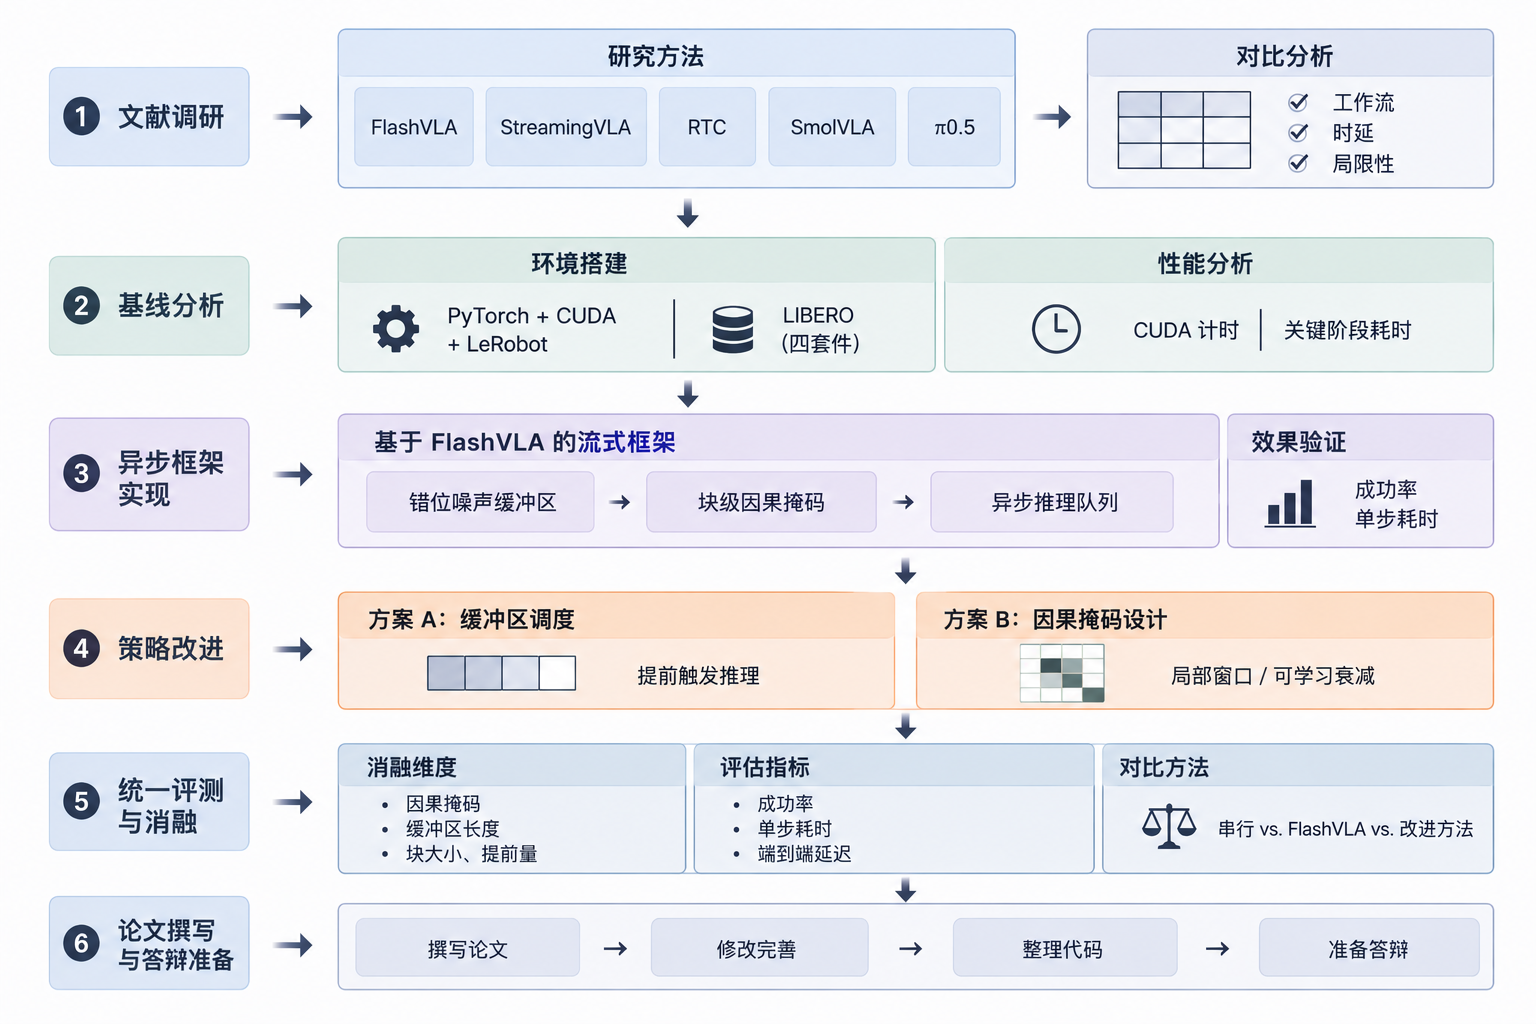
\includegraphics[width=0.8\textwidth]{figures/tech_route.png}\\[6pt]
    {\zihao{5} 图1\quad 技术路线图}
\end{center}

\textbf{可行性分析：}

\begin{itemize}
  \item \textbf{理论可行性：}FlashVLA的块级因果注意力与错位噪声缓冲已有明确形式化描述和消融验证。
  \item \textbf{技术可行性：}\(\pi_{0.5}\)与FlashVLA均有开源实现与适配权重；LIBERO提供标准化数据组织、观测接口、动作空间与评测脚本；分阶段计时可用CUDA事件与Python打点实现。
  \item \textbf{资源可行性：}实验室具备充足的GPU资源，实验以仿真验证为主，真机测试视条件开展。
  \item \textbf{风险与应对：}（a）复现精度不及论文——优先使用官方权重与配置，若存在差异则记录并分析原因，将复现偏差本身作为分析对象；（b）改进方向效果不佳——转为系统性的配置敏感性分析，仍可形成有价值的实验贡献；（c）实验结果受仿真渲染干扰——区分仿真时间与实际运行时间，将渲染与通信单独计时。
\end{itemize}

\tjformsubsection{3．工作进度安排}
\begin{center}
  \captionof*{table}{表1\quad 工作进度安排}
  \begin{tabularx}{\linewidth}{@{}lX@{}}
    \toprule
    \textbf{周次} & \textbf{工作内容} \\
    \midrule
    第1—4周   & 开展VLA、动作分块、异步推理及流式动作生成相关文献调研，学习RTC、StreamingVLA、FlashVLA等代表性方法，熟悉机器人操作仿真任务，明确研究范围并完成开题准备。 \\
    第5—8周   & 搭建仿真与模型运行环境，运行适配任务的预训练模型（\(\pi_{0.5}\)），建立串行推理与控制基线。 \\
    第9—12周  & 完成分阶段计时与运行时间线分析，确定异步流水线方案及评价指标。 \\
    第13—18周 & FlashVLA复现。实现错位噪声缓冲区、块级因果注意力、冷启动与稳态推理循环；完成多缓冲区联合微调的数据打包；在LIBERO d=1下验证成功率与延迟，对照论文数据。 \\
    第19—24周 & 研究改进策略，完成至少一种改进方法的实现与验证。 \\
    第25—27周 & 在仿真环境中开展消融实验，并比较串行执行、FlashVLA异步框架及所提改进方法。 \\
    第28—30周 & 整理实验结果、系统流程图及分析图表，完成毕业论文初稿，完善代码、配置文件和复现实验说明。 \\
    第31—32周 & 根据指导意见修改完善毕业论文，完成最终材料提交和毕业答辩准备。 \\
    \bottomrule
  \end{tabularx}
\end{center}

\tjformsection{三、\tjheadertext 主要参考文献}

% 参考文献条目：与正文同字号、同颜色（不用 \tjformhint 的灰色提示样式）
\newcommand{\tjproprev}[1]{{\tjfontbody\selectfont #1\par}}

\tjproprev{[1] Li Z., Tang J., Liu Z. FlashVLA: Streaming Action Decoding for Fast and Asynchronous VLA Inference. arXiv:2608.27384.}

\tjproprev{[2] Shi Y., Guo D., Zhao T., et al. StreamingVLA: Streaming Vision-Language-Action Model with Action Flow Matching and Adaptive Early Observation. arXiv:2603.28565.}

\tjproprev{[3] Black K., Brown N., Driess D., et al. \(\pi_0\): A Vision-Language-Action Flow Model for General Robot Control. RSS, 2025. arXiv:2410.24164.}

\tjproprev{[4] Physical Intelligence, Black K., Brown N., et al. \(\pi_{0.5}\): A Vision-Language-Action Model with Open-World Generalization. arXiv:2504.16054.}

\tjproprev{[5] Kim M. J., Pertsch K., Karamcheti S., et al. OpenVLA: An Open-Source Vision-Language-Action Model. arXiv:2406.09246.}

\tjproprev{[6] Black K., Galliker M. Y., Levine S. Real-Time Execution of Action Chunking Flow Policies. NeurIPS, 2025. arXiv:2506.07339.}

\tjproprev{[7] Shukor M., Aubakirova D., Capuano F., et al. SmolVLA: A Vision-Language-Action Model for Affordable and Efficient Robotics. arXiv:2506.01844.}

\tjproprev{[8] Jiang S., Fang X., Roy N., et al. Streaming Flow Policy: Simplifying Diffusion/Flow-Matching Policies by Treating Action Trajectories as Flow Trajectories. CoRL, 2025. arXiv:2505.21851.}

\tjproprev{[9] Liu B., Zhu Y., Gao C., et al. LIBERO: Benchmarking Knowledge Transfer for Lifelong Robot Learning. NeurIPS, 2023, 36: 44776-44791.}

\tjproprev{[10] J. Tang, Y. Sun, Y. Zhao, S. Yang, Y. Lin, Z. Zhang, J. Hou, Y. Lu, Z. Liu, and S. Han. VLaSH: Real-time VLAs via Future-State-Aware Asynchronous Inference, 2025. arXiv:2512.01031.}

\tjproprev{[11] B. Chen, D. M. Monso, Y. Du, M. Simchowitz, R. Tedrake, and V. Sitzmann. Diffusion Forcing: Next-token Prediction Meets Full-Sequence Diffusion, 2024. arXiv:2407.01392.}

\tjproprev{[12] A. Kodaira, T. Hou, J. Hou, M. Georgopoulos, F. Juefei-Xu, M. Tomizuka, and Y. Zhao. StreamDiT: Real-time Streaming Text-to-Video Generation, 2026. arXiv:2507.03745.}

\tjformsection{四、审核意见}

\begin{tjreviewbox}
  \tjformlabel{指导教师意见：}\tjformhint{（课题难度是否适中、工作量是否饱满、进度安排是否合理、工作条件是否具备、是否同意开题等）}

  \vspace{8\baselineskip}
  \tjformsignature{指导教师签名}{8em}
\end{tjreviewbox}

\begin{tjreviewbox}
  \tjformlabel{专业审核意见：}\tjformhint{（适当对各项内容给与意见和评价，字数不限。）}

  \vspace{6\baselineskip}
  \tjformsignature{负责人签名}{8em}
\end{tjreviewbox}